% Specifically, we develop recipes to find suitable designs of association studies such that combination of the dimensionality $p$, sparsity $\beta$, and signal sizes $r$ of the problem lands in the desired region of risk control, as predicted by the results in Section \ref{sec:chisq-boundaries}.

% Of course, in applications, not all three of the parameters $(p, \beta, r)$ can be altered as we wish.
% In particular, the problem dimensions and sparsity levels are usually determined by the underlying physical processes.
% In the GWAS example, the number of genomic marker locations is determined by the chip used for gene sequencing, while the number of relevant genomic locations is a consequence of the biological process.
% Therefore, in order to achieve a desired level of error control, we can often only hope to influence the statistical signal sizes.

Returning to the problem of \emph{high-dimensional} marginal screenings for categorical covariates, we explore the manifestation of the phase transition in the exact-approximate support recovery problem in the genetic context.

Recall Theorem \ref{thm:chi-squared-exact-approx-boundary} predicts that FWER and FNR can be simultaneously controlled in large dimensions if and only if 
\begin{equation}
    r = \frac{\lambda}{2\log{p}} = \frac{w^2n}{2\log{p}} > 1.
\end{equation}
Therefore, if we were to apply FWER-controlling procedures at low nominal levels (say, $5\%$), then the FNR would experience a phase transition
in the following sense.  If the signal size is strong enough, i.e., 
\begin{equation} \label{eq:power-1-region}
    r>1 \iff w^2 > \frac{2\log{p}}{n},
\end{equation}
then the FNR can be close to 0; otherwise, FNR must be close to 1.

% Translating this result into the language of association tests, 
Using the parametric relationship described in Corollary \ref{cor:signal-size-odds-ratio-conditional-frequency} (and Proposition \ref{prop:signal-size-odds-ratio}), 
the inequalities in \eqref{eq:power-1-region} implicitly define regions of $(f, R)$ where associations are discoverable with high power, for a given $\phi_1$.
Further, the boundary of such discoverable regions sharpens as dimensionality diverges. 
We illustrate this phase transition through a numerical example next.


\begin{figure}
      \centering
      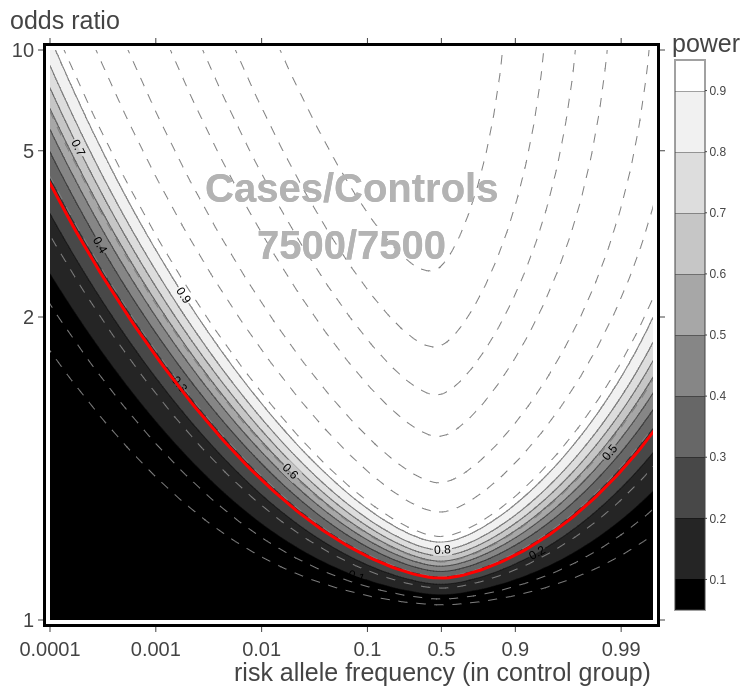
\includegraphics[width=0.49\textwidth]{OR-RAF_plots/OR-RAF_p4.png} 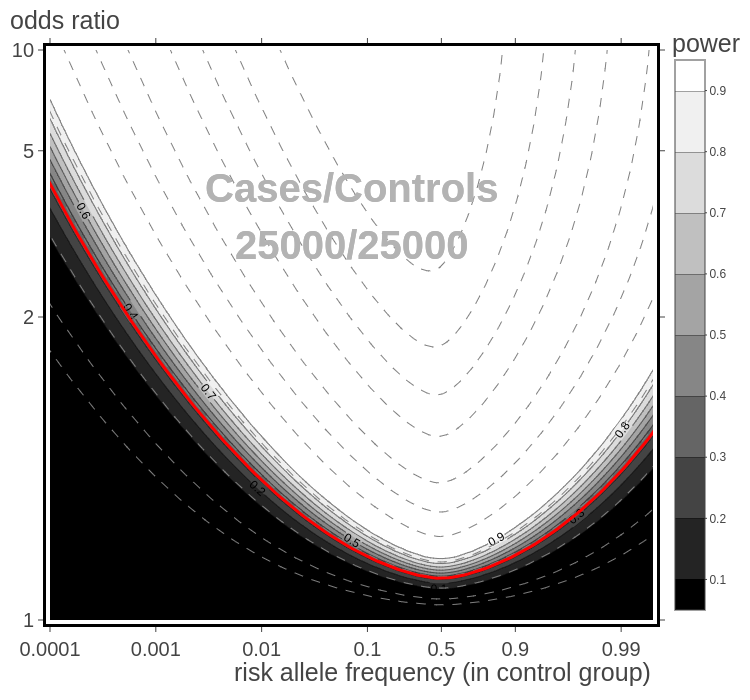
\includegraphics[width=0.49\textwidth]{OR-RAF_plots/OR-RAF_p1e2.png} 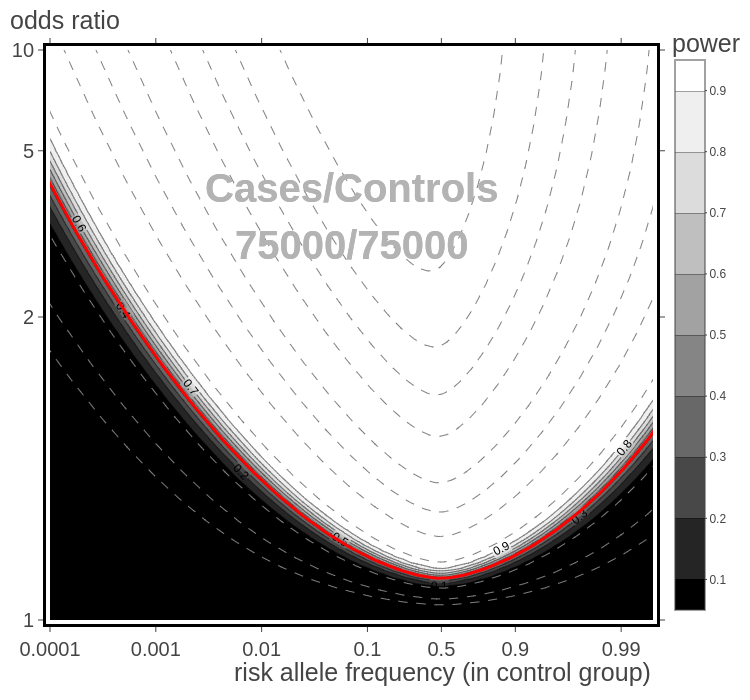
\includegraphics[width=0.49\textwidth]{OR-RAF_plots/OR-RAF_p1e6.png} 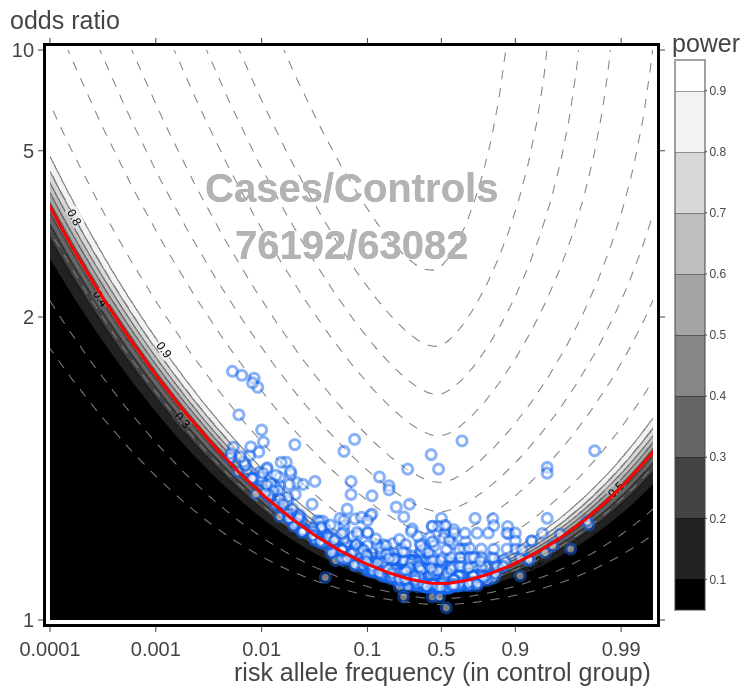
\includegraphics[width=0.49\textwidth]{OR-RAF_plots/OR-RAF_BC_study.png}
      \caption{The OR-RAF diagram visualizing the marginal power of discovery in genetic association studies, after applying Bonferroni's procedure with nominal FWER at $5\%$ level. Sample sizes are marked in each panel, and the problem dimensions are, respectively, $p=4$ (upper-left), $p=10^2$ (upper-right), and $p=10^6$ (lower-left), so that $n/\log{p}$ are roughly constant. Red curves mark the boundaries ($r=1$) of the phase transition for the exact-approximate support recovery problem; dashed curves are the equi-signal (equi-power) curves. The phase transition in signal sizes $\lambda$ translates into the phase transition in terms of $(f,R)$, and sharpens as $p\to\infty$; see Example \ref{exmp:OR-RAF_phase_transition}. In the lower-right panel, we visualize discovered associations (blue circles) in a recent GWA study (Michailidou et al. (2017)); the estimated odds ratios and risk allele frequencies are subject to survival bias and should not be taken at their face values; see Remark \ref{rmk:OR-RAF_false_evidence}.
      } 
      \label{fig:OR-RAF_GWAS}
\end{figure}


\begin{example}
\label{exmp:OR-RAF_phase_transition}
Consider association tests on $2\times2$ contingency tables at $p$ locations as introduced in Section \ref{sec:motivation-chisq}, where the counts follow 
a multinomial distribution
% independent binomial distributions 
% $$
% O_{11} \sim \mathrm{Binom}(n\phi_1, fR/(fR+1-f)),\quad 
% O_{21} \sim \mathrm{Binom}(n(1-\phi_1), fR/(fR+1-f)),
% $$
parametrized by $(f, R, \phi_1)$ as in Section \ref{sec:optimal-design}.
Assume that the phenotype marginals are fixed at $\phi_1 = \phi_2 = 1/2$.
% --- as is the case in genetic association studies --- 
Applying Bonferroni's procedure with nominal FWER at $\alpha=5\%$ level, we can approximate the marginal power of association tests by
\begin{equation} \label{eq:power-approximation}
    \P[\chi^2_{1}(\lambda)>\chi^2_{1,\alpha/p}],
\end{equation}
where $\chi^2_{1,\alpha/p}$ is the upper $(\alpha/p)$-quantile of a central chi-squared distribution with 1 degree of freedom.
We calculate this marginal power as a function of the parameters $(f,R)$ in three scenarios:
\begin{itemize}
    \item $p=4$, $n=3\times10^4$ 
    \item $p=10^2$, $n=1\times10^5$
    \item $p=10^6$, $n=3\times10^6$
\end{itemize}
and visualize the results as heatmaps\footnote{Since genetic variants can always be relabelled such that Variant 1 is positively associated with Cases, we only produce part of the diagram where $R>1$.
Sample sizes marked in the figure are adjusted by a factor of $1/2$, to reflect the genetic context where a pair of alleles are measured for every individual at every genomic location.} (referred to as OR-RAF diagrams) in Figure \ref{fig:OR-RAF_GWAS}.
These parameter values are chosen so that $\log(p)/n$ are roughly constant (around $4.6\times10^{-5}$).

We also overlay ``equi-signal'' curves, i.e., functions implicitly defined by the equations $r=c$ for a range of $c$ (dashed curves), and highlight the predicted boundary of phase transition for the exact-approximate support recovery problem $r=1$ (red curves).
The change in marginal power clearly sharpens around the predicted boundary $r=1$ as dimensionality diverges.
\end{example}

% --- or equivalently, the marginal power ---


\begin{remark}
\label{rmk:OR-RAF_false_evidence}
In an attempt to find empirical evidence of our theoretical predictions, we chart the genetic variants associated with breast cancer, discovered in a 2017 study by \citet{michailidou2017association} in an OR-RAF diagram. 
The estimated risk allele frequencies ($f$) and odds ratios ($R$) are taken from the NHGRI-EBI GWAS catalog \cite{macarthur2016new}, and plotted against a power heatmap calculated according to the reported sample sizes. 
See lower-right panel of Figure \ref{fig:OR-RAF_GWAS}.

It is tempting to believe, on careless inspection, that roughly \emph{all} discovered associations fall inside the high power region of the diagram, therefore demonstrating the phase transition in statistical power.
Unfortunately, the estimates here are subject to survival {bias} --- the study in fact uses the {same} dataset for \emph{both} support estimation and parameter estimation, without adjusting the latter for the selection process.
The seemingly striking agreement between the power calculations and the estimated effects of reported associations \emph{should not} be taken as evidence for the validity of our theory.
We conjecture, as the theory predicts, that accurate and unbiased parameter estimates from an independent replication will still place the associations in the high power region of the diagram. 
\end{remark}

Finally, we demonstrate with an example how results in Sections \ref{sec:chisq-boundaries} and \ref{sec:odds-and-power} may be used for planning prospective association studies.

\begin{example}
In a GWAS with $p = 10^6$ genomic marker locations, researchers wish to locate genetic associations with the trait of interest.
Specifically, they wish to maximize power in the region where genetic variants have risk allele frequencies of $0.01$ and odds ratios of $1.2$.
By Corollary \ref{cor:optimal-design}, the optimal design has a fraction of cases $\phi^* = 0.478$, yielding the statistical signal size per sample $w^2\approx9.00\times10^{-5}$ according to Corollary \ref{cor:signal-size-odds-ratio-conditional-frequency}.

If we wish to achieve exact-approximate support recovery in the sense of \eqref{eq:support-recovery-success}, Theorem \ref{thm:chi-squared-exact-approx-boundary} predicts that the signal size parameter $r$ has to be at least $f_{\mathrm{EA}}(\beta)= 1$.
This signal size calls for a sample size of $n = \lambda / w^2 = 2r\log(p)/w^2 \approx 307,011$.
In a typical GWAS, a pair of alleles are sequenced for every marker location, bringing the required number of subjects in the study to $n/2 \approx 153,509$.
\end{example}

In comparison, a more accurate power calculation directly using \eqref{eq:power-approximation} predicts that $n / 2 = 165,035$ subjects are needed, under the set of parameters ($p=10^6$, $f=0.01$, $R=1.2$) and $\mathrm{FWER}=0.05$, $\mathrm{FNR}=0.5$; this is $7\%$ higher than our crude asymptotic approximation.
% The accuracy of the asymptotic approximations, by nature of the statements in Theorem \ref{thm:chi-squared-exact-boundary} and \ref{thm:chi-squared-approx-boundary}, depends on how close the error metrics are to zero.
% For example, the number of subjects needed for $\mathrm{FWER}=\mathrm{FWNR}=0.01$ is $499,598$, an $8\%$ increase over the asymptotic prediction; at $\mathrm{FWER}=\mathrm{FWNR}=0.1$, this number becomes $398,996$, some $14\%$ lower than the asymptotic result.
In general, we recommend using the more precise calculations over the back-of-the-envelope asymptotics for planning prospective studies and performing systematic reviews;
a user-friendly web application implementing the more precise approximations is provided in \cite{gao2019upass}.
Nevertheless, the theoretical results on phase transitions generate simple, accurate, and powerful insights that cannot be easily derived from numerical calculations.

